% Generated by make_figure.py - do not edit by hand.
\begin{figure}[!ht]
\centering
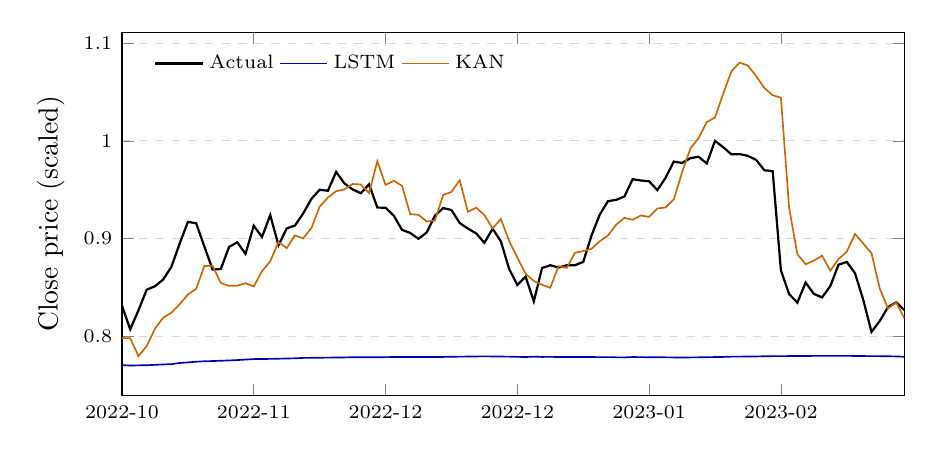
\begin{tikzpicture}
\begin{axis}[
  width=0.95\textwidth, height=6.2cm,
  xmin=0, xmax=95, ylabel={Close price (scaled)},
  xtick={0,16,32,48,64,80},
  xticklabels={2022-10,2022-11,2022-12,2022-12,2023-01,2023-02},
  x tick label style={font=\scriptsize},
  y tick label style={font=\scriptsize},
  legend style={font=\scriptsize, draw=none}, legend pos=north west,
  legend columns=3, ymajorgrids, grid style={dashed,gray!30}]
\addplot+[mark=none, thick, black] coordinates {
(0,0.8314) (1,0.8072) (2,0.8267) (3,0.8478) (4,0.8513) (5,0.8582) (6,0.8712) (7,0.8949) (8,0.9171) (9,0.9158) (10,0.8920) (11,0.8684) (12,0.8689) (13,0.8916) (14,0.8963) (15,0.8845) (16,0.9132) (17,0.9017) (18,0.9241) (19,0.8933) (20,0.9105) (21,0.9134) (22,0.9258) (23,0.9407) (24,0.9500) (25,0.9490) (26,0.9683) (27,0.9566) (28,0.9503) (29,0.9465) (30,0.9556) (31,0.9318) (32,0.9316) (33,0.9235) (34,0.9090) (35,0.9058) (36,0.8998) (37,0.9064) (38,0.9235) (39,0.9313) (40,0.9293) (41,0.9160) (42,0.9103) (43,0.9054) (44,0.8957) (45,0.9102) (46,0.8972) (47,0.8692) (48,0.8526) (49,0.8611) (50,0.8359) (51,0.8699) (52,0.8728) (53,0.8705) (54,0.8728) (55,0.8728) (56,0.8762) (57,0.9030) (58,0.9245) (59,0.9383) (60,0.9397) (61,0.9431) (62,0.9608) (63,0.9595) (64,0.9587) (65,0.9496) (66,0.9623) (67,0.9789) (68,0.9774) (69,0.9823) (70,0.9838) (71,0.9769) (72,1.0000) (73,0.9935) (74,0.9862) (75,0.9865) (76,0.9847) (77,0.9805) (78,0.9699) (79,0.9691) (80,0.8676) (81,0.8432) (82,0.8346) (83,0.8551) (84,0.8435) (85,0.8399) (86,0.8515) (87,0.8734) (88,0.8762) (89,0.8646) (90,0.8374) (91,0.8046) (92,0.8158) (93,0.8299) (94,0.8349) (95,0.8268)};
\addplot+[mark=none, semithick, blue!70!black] coordinates {
(0,0.7706) (1,0.7702) (2,0.7704) (3,0.7705) (4,0.7709) (5,0.7713) (6,0.7716) (7,0.7728) (8,0.7734) (9,0.7741) (10,0.7746) (11,0.7748) (12,0.7751) (13,0.7754) (14,0.7758) (15,0.7763) (16,0.7768) (17,0.7769) (18,0.7770) (19,0.7772) (20,0.7774) (21,0.7776) (22,0.7780) (23,0.7781) (24,0.7782) (25,0.7783) (26,0.7784) (27,0.7785) (28,0.7787) (29,0.7787) (30,0.7786) (31,0.7786) (32,0.7788) (33,0.7789) (34,0.7789) (35,0.7789) (36,0.7789) (37,0.7790) (38,0.7790) (39,0.7790) (40,0.7792) (41,0.7793) (42,0.7794) (43,0.7795) (44,0.7796) (45,0.7795) (46,0.7794) (47,0.7793) (48,0.7791) (49,0.7789) (50,0.7793) (51,0.7790) (52,0.7791) (53,0.7789) (54,0.7789) (55,0.7789) (56,0.7789) (57,0.7789) (58,0.7788) (59,0.7788) (60,0.7786) (61,0.7785) (62,0.7789) (63,0.7788) (64,0.7787) (65,0.7787) (66,0.7786) (67,0.7785) (68,0.7785) (69,0.7785) (70,0.7786) (71,0.7787) (72,0.7789) (73,0.7790) (74,0.7793) (75,0.7793) (76,0.7795) (77,0.7795) (78,0.7797) (79,0.7798) (80,0.7798) (81,0.7799) (82,0.7799) (83,0.7799) (84,0.7801) (85,0.7801) (86,0.7801) (87,0.7801) (88,0.7801) (89,0.7800) (90,0.7799) (91,0.7798) (92,0.7798) (93,0.7797) (94,0.7795) (95,0.7792)};
\addplot+[mark=none, semithick, orange!80!black] coordinates {
(0,0.7984) (1,0.7981) (2,0.7799) (3,0.7900) (4,0.8079) (5,0.8191) (6,0.8242) (7,0.8329) (8,0.8429) (9,0.8485) (10,0.8720) (11,0.8722) (12,0.8546) (13,0.8517) (14,0.8519) (15,0.8544) (16,0.8511) (17,0.8667) (18,0.8768) (19,0.8966) (20,0.8903) (21,0.9034) (22,0.9003) (23,0.9109) (24,0.9327) (25,0.9420) (26,0.9485) (27,0.9503) (28,0.9559) (29,0.9554) (30,0.9467) (31,0.9792) (32,0.9549) (33,0.9592) (34,0.9541) (35,0.9250) (36,0.9244) (37,0.9175) (38,0.9187) (39,0.9448) (40,0.9478) (41,0.9598) (42,0.9274) (43,0.9317) (44,0.9242) (45,0.9104) (46,0.9201) (47,0.8977) (48,0.8807) (49,0.8642) (50,0.8567) (51,0.8528) (52,0.8498) (53,0.8719) (54,0.8701) (55,0.8856) (56,0.8873) (57,0.8896) (58,0.8973) (59,0.9032) (60,0.9143) (61,0.9213) (62,0.9194) (63,0.9237) (64,0.9222) (65,0.9309) (66,0.9319) (67,0.9402) (68,0.9678) (69,0.9921) (70,1.0028) (71,1.0193) (72,1.0240) (73,1.0484) (74,1.0713) (75,1.0802) (76,1.0769) (77,1.0662) (78,1.0541) (79,1.0467) (80,1.0443) (81,0.9314) (82,0.8840) (83,0.8738) (84,0.8775) (85,0.8826) (86,0.8673) (87,0.8791) (88,0.8867) (89,0.9048) (90,0.8950) (91,0.8850) (92,0.8491) (93,0.8285) (94,0.8347) (95,0.8184)};
\legend{Actual, LSTM, KAN}
\end{axis}
\end{tikzpicture}
\caption{TODO write caption}
\label{fig:figure_h100_step1_s0_pykan}
\end{figure}
